%
% Coverage study of deltaCP
% 

{\huge{Update}}
\section{Coverage study of the simultaneous fit of $\delta_{CP}$ and mass hierarchy}
\label{sec:coverage_deltacp}


The flux tuning for the antineutrino mode samples corresponds to the full Run 1-7c data set.
So we can safely state that the calculation of the $\Delta \chi^2$ critical values will not be affected 
by this change.

In \cref{tab:critval_0_pmhalfpi_run17c} the critical values and the coverage is shown for the following values
of $\delta_{CP}$ and mass hierarchy: $-\pi/2$, 0, $+\pi/2$ and normal hierarchy.
In \cref{fig:dchisq_bestfit_dcp_run17c} the expected distributions of $\Delta \chi^2$   
and best-fit $\delta_{CP}$ are shown. 

\begin{table}
\center
\begin{tabular}{| c | c | c |}
\hline
 \multicolumn{3}{| c |}{\bf Gaussian approximation}  \\
\hline
    {\bf CL} & \multicolumn{2}{c |}{\bf Critical value}  \\
\hline
\multicolumn{1}{| c |}{$1\sigma$}& \multicolumn{2}{| c |}{1}  \\ \hline
\multicolumn{1}{| c |}{90\%}& \multicolumn{2}{| c |}{2.71}  \\ \hline
\multicolumn{1}{| c |}{$2\sigma$}& \multicolumn{2}{| c |}{4}  \\ \hline
\hline
\multicolumn{3}{| c | }{{\bf Feldman-Cousins:} $\delta^{true}_{CP} = -\pi/2$, $MH^{true} = \text{normal}$}  \\
\hline
    {\bf CL} & {\bf Critical value} &{\bf Coverage}  \\
\hline
$1\sigma$& $0.588$ & 0.774 \\ \hline
90\%& $2.106$ & 0.935\\ \hline
$2\sigma$& $3.285$& 0.972 \\ \hline
\hline
\multicolumn{3}{| c | }{{\bf Feldman-Cousins:} $\delta^{true}_{CP} = 0$, $MH^{true} = \text{normal}$}  \\
\hline
    {\bf CL}& {\bf Critical value} &{\bf Coverage}  \\
\hline
$1\sigma$& $1.374$ & 0.564 \\ \hline
90\%& $2.576$ & 0.913     \\ \hline
$2\sigma$& $3.387$ & 0.973\\ \hline
\hline
\multicolumn{3}{| c | }{{\bf Feldman-Cousins:} $\delta^{true}_{CP} = +\pi/2$, $MH^{true} = \text{normal}$}  \\
\hline
    {\bf CL} & {\bf Critical value} &{\bf Coverage}  \\
\hline
$1\sigma$& $1.257$ & 0.578 \\ \hline
90\%& $2.375$ & 0.928 \\ \hline
$2\sigma$& $3.254$ & 0.974\\ \hline
\end{tabular}
\caption{
The critical values of $\Delta \chi^2$ used to set the confidence intervals are shown
for both the gaussian approximation (i.e. constant $\Delta \chi^2$) as
well as the ones obtained with the Feldman-Cousins method.
10k toy experiments were used for each true point of $\delta_{CP}$.
Furthermore the coverage, defined by \cref{eq:coverage},
provided by the gaussian approximation for different true values $\delta_{CP}$ is shown.
The true mass hierarchy is set to normal.
The collected statistic corresponds to the Run 1-7c data set one.
%The errors on the critical values are computed using \cref{eq:def_crit_val_error}
}             
\label{tab:critval_0_pmhalfpi_run17c}                                                                                                                                                                             
\end{table}


\begin{figure*}[htb]
\center
\begin{subfigure}[b]{0.49\textwidth}
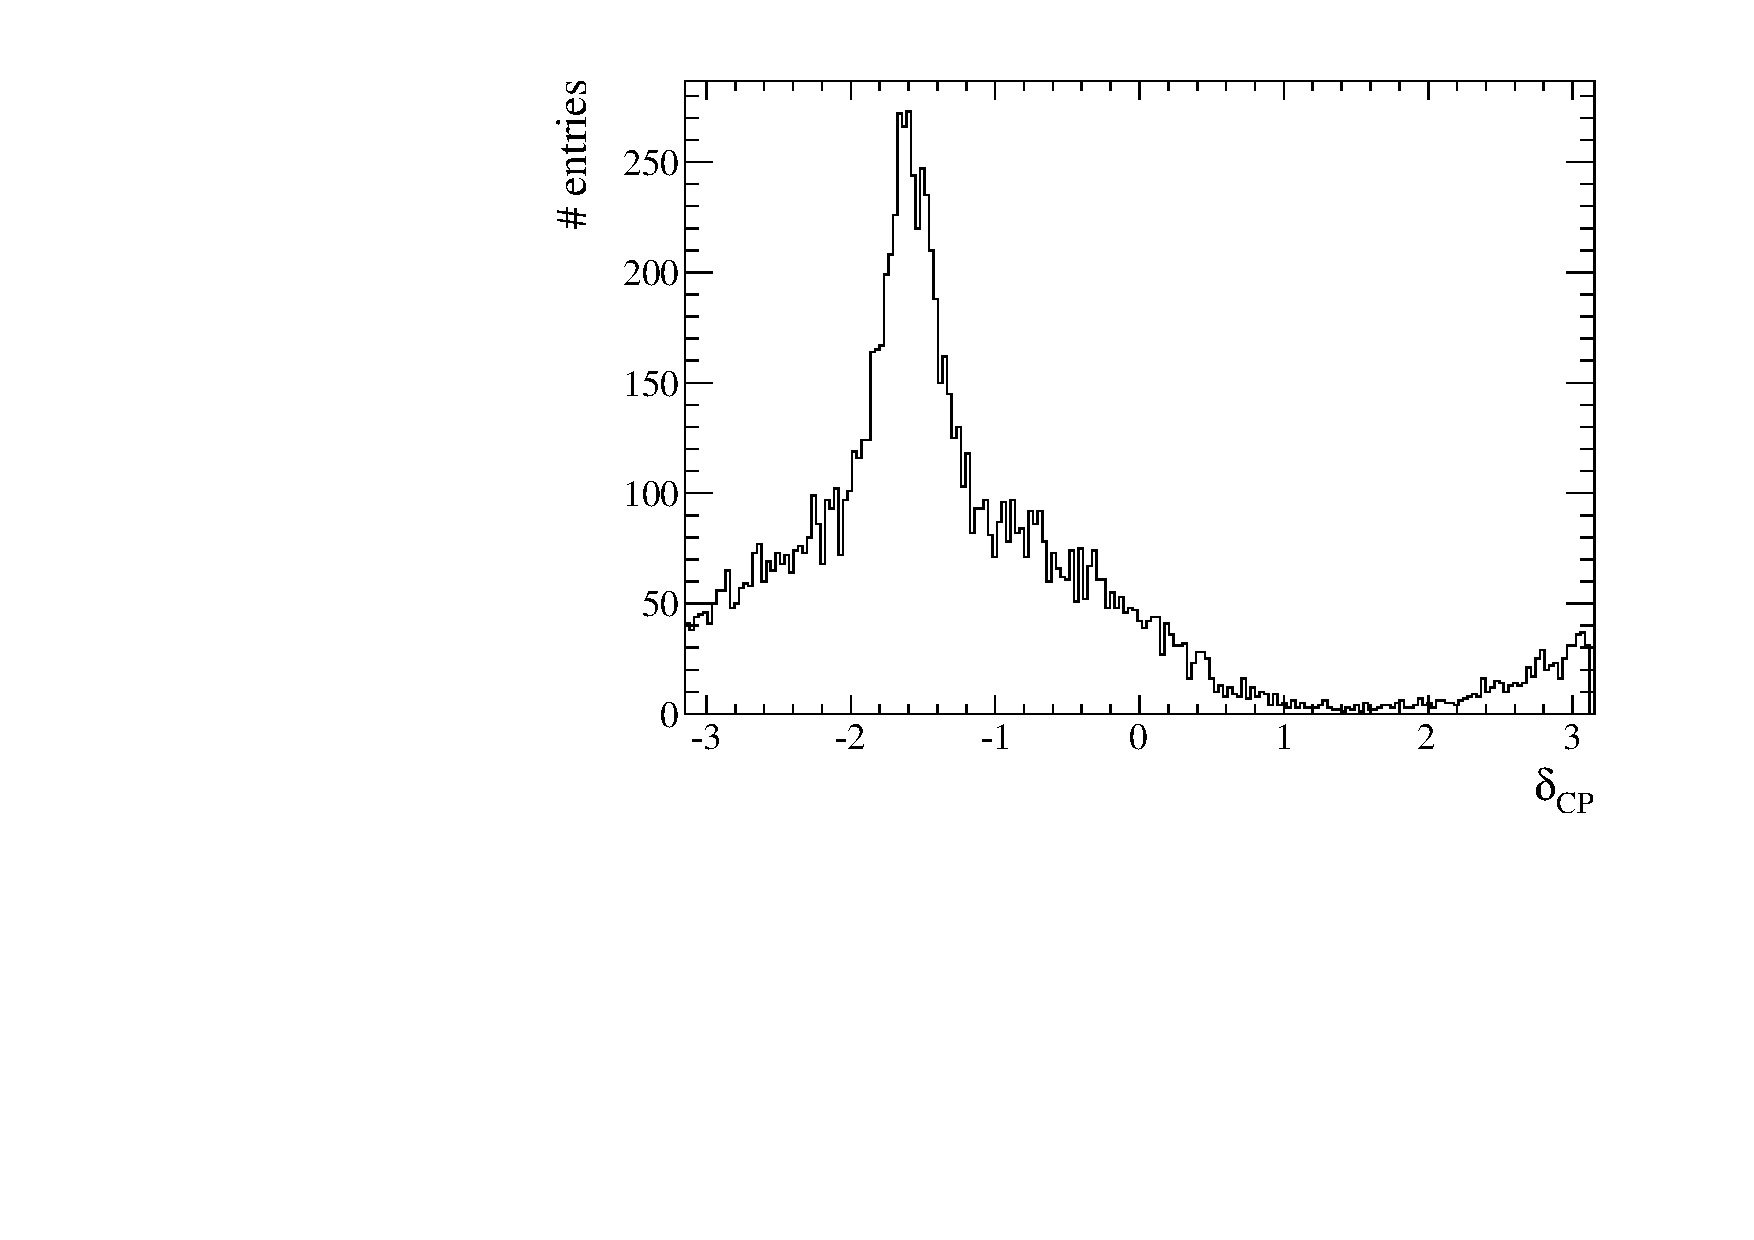
\includegraphics[width=0.9\textwidth]{./joint_plots/coverage_fc/coverage_run17c/Run17_cbestfit_deltacp_m1p571_normal.pdf}
\caption{Best-fit distribution of $\delta_{CP}$. $\delta_{CP}^{true} = -\pi/2$.}
\end{subfigure}
\begin{subfigure}[b]{0.49\textwidth}
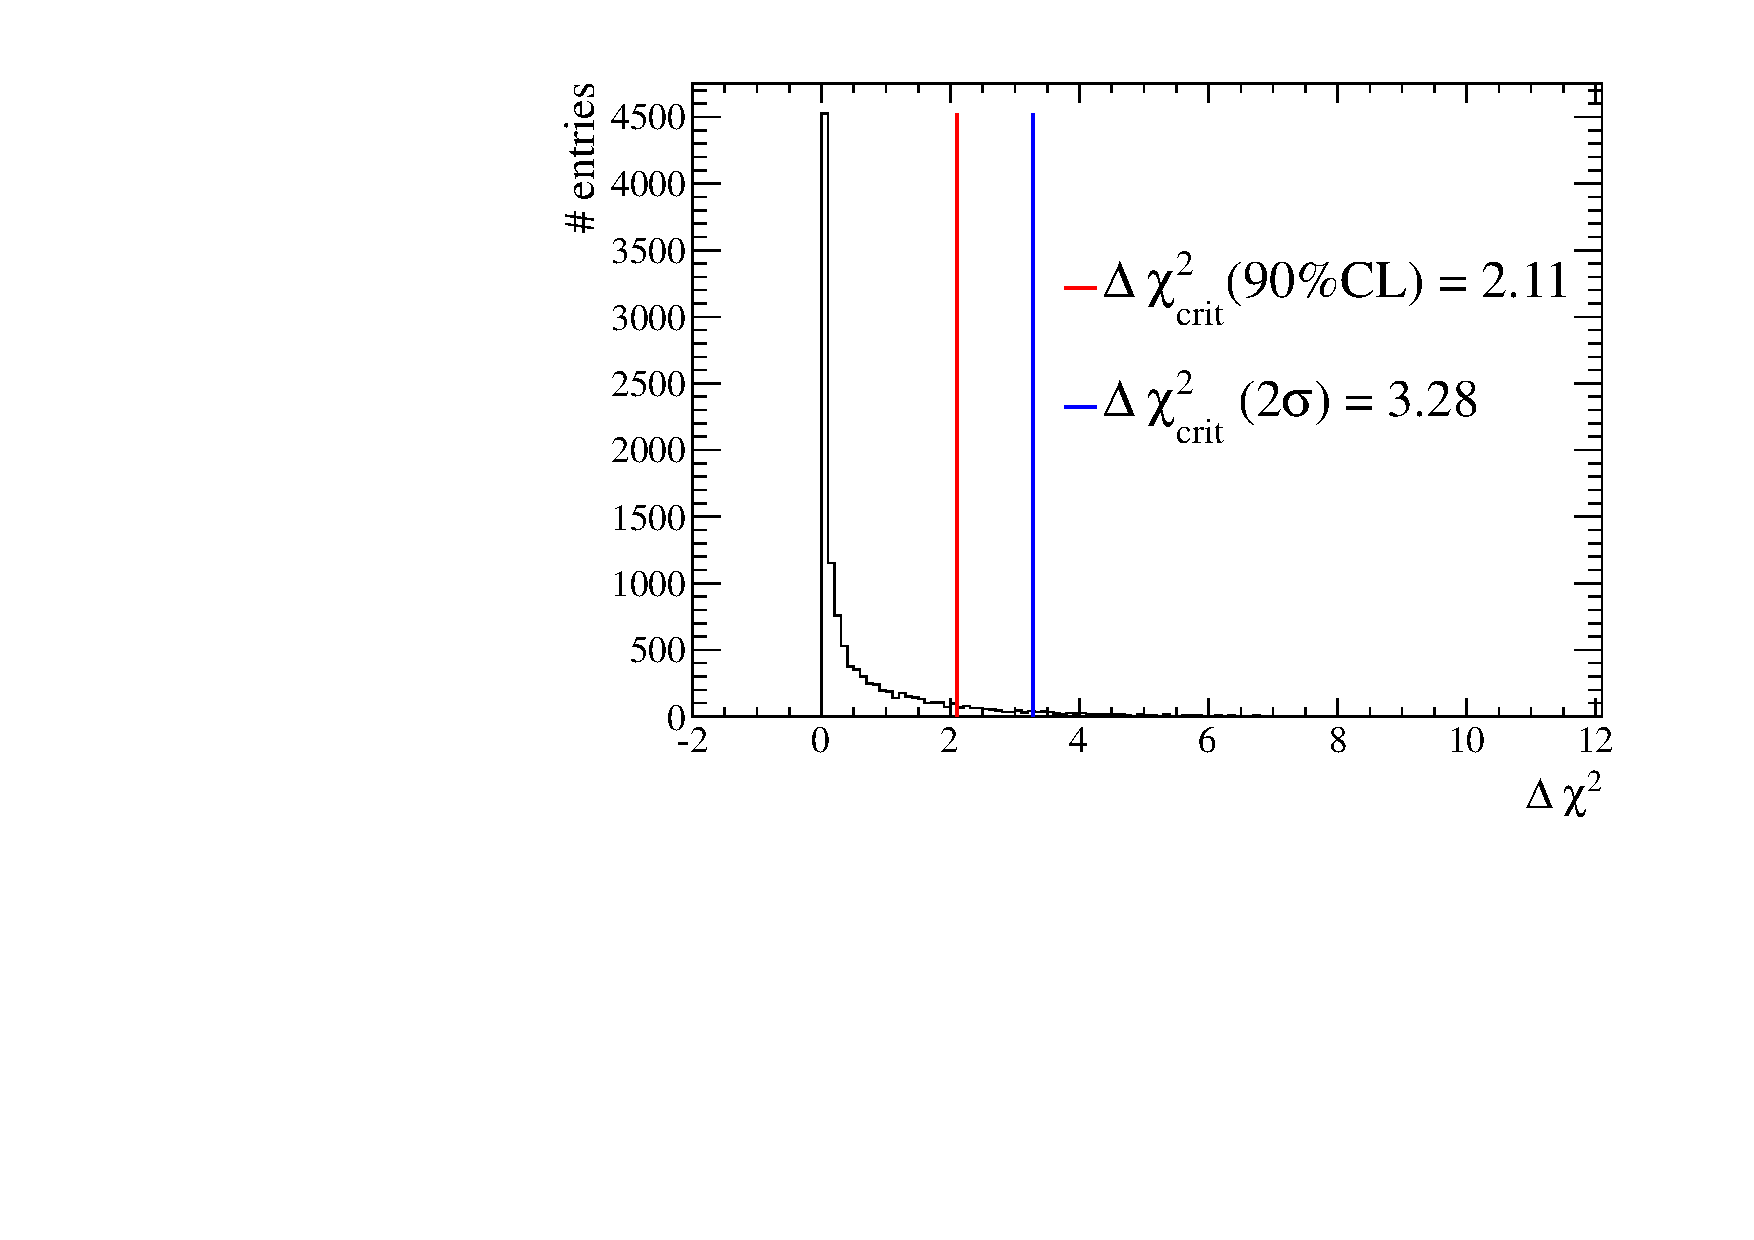
\includegraphics[width=0.9\textwidth]{./joint_plots/coverage_fc/coverage_run17c/Run17_deltachisq_glob_deltacp_m1p571_normal.pdf}
\caption{$\Delta \chi^2$ distribution.
$\delta_{CP}^{true} = -\pi/2$.}
\end{subfigure}
\begin{subfigure}[b]{0.49\textwidth}
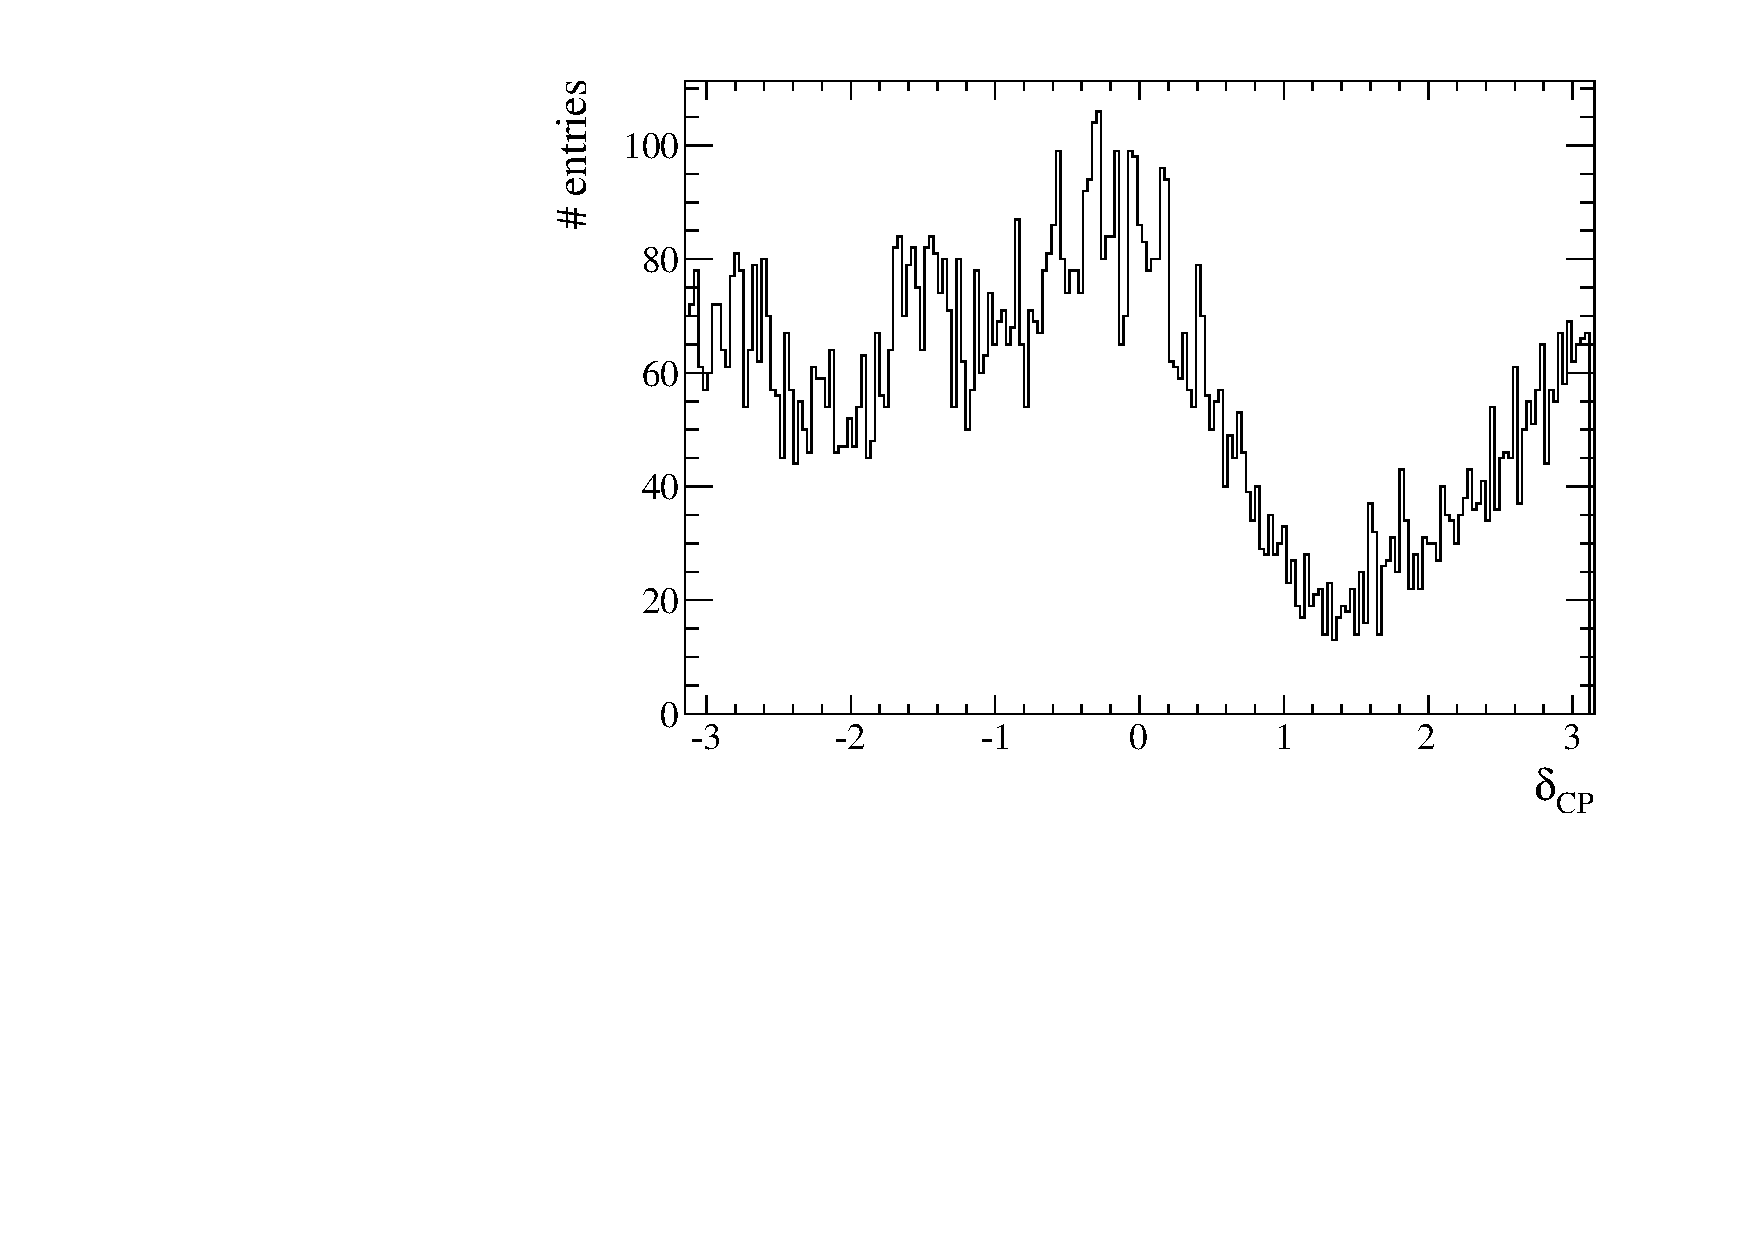
\includegraphics[width=0.9\textwidth]{./joint_plots/coverage_fc/coverage_run17c/Run17_cbestfit_deltacp_0_normal.pdf}
\caption{Best-fit distribution of $\delta_{CP}$. $\delta_{CP}^{true} = 0$.}
\end{subfigure}
\begin{subfigure}[b]{0.49\textwidth}
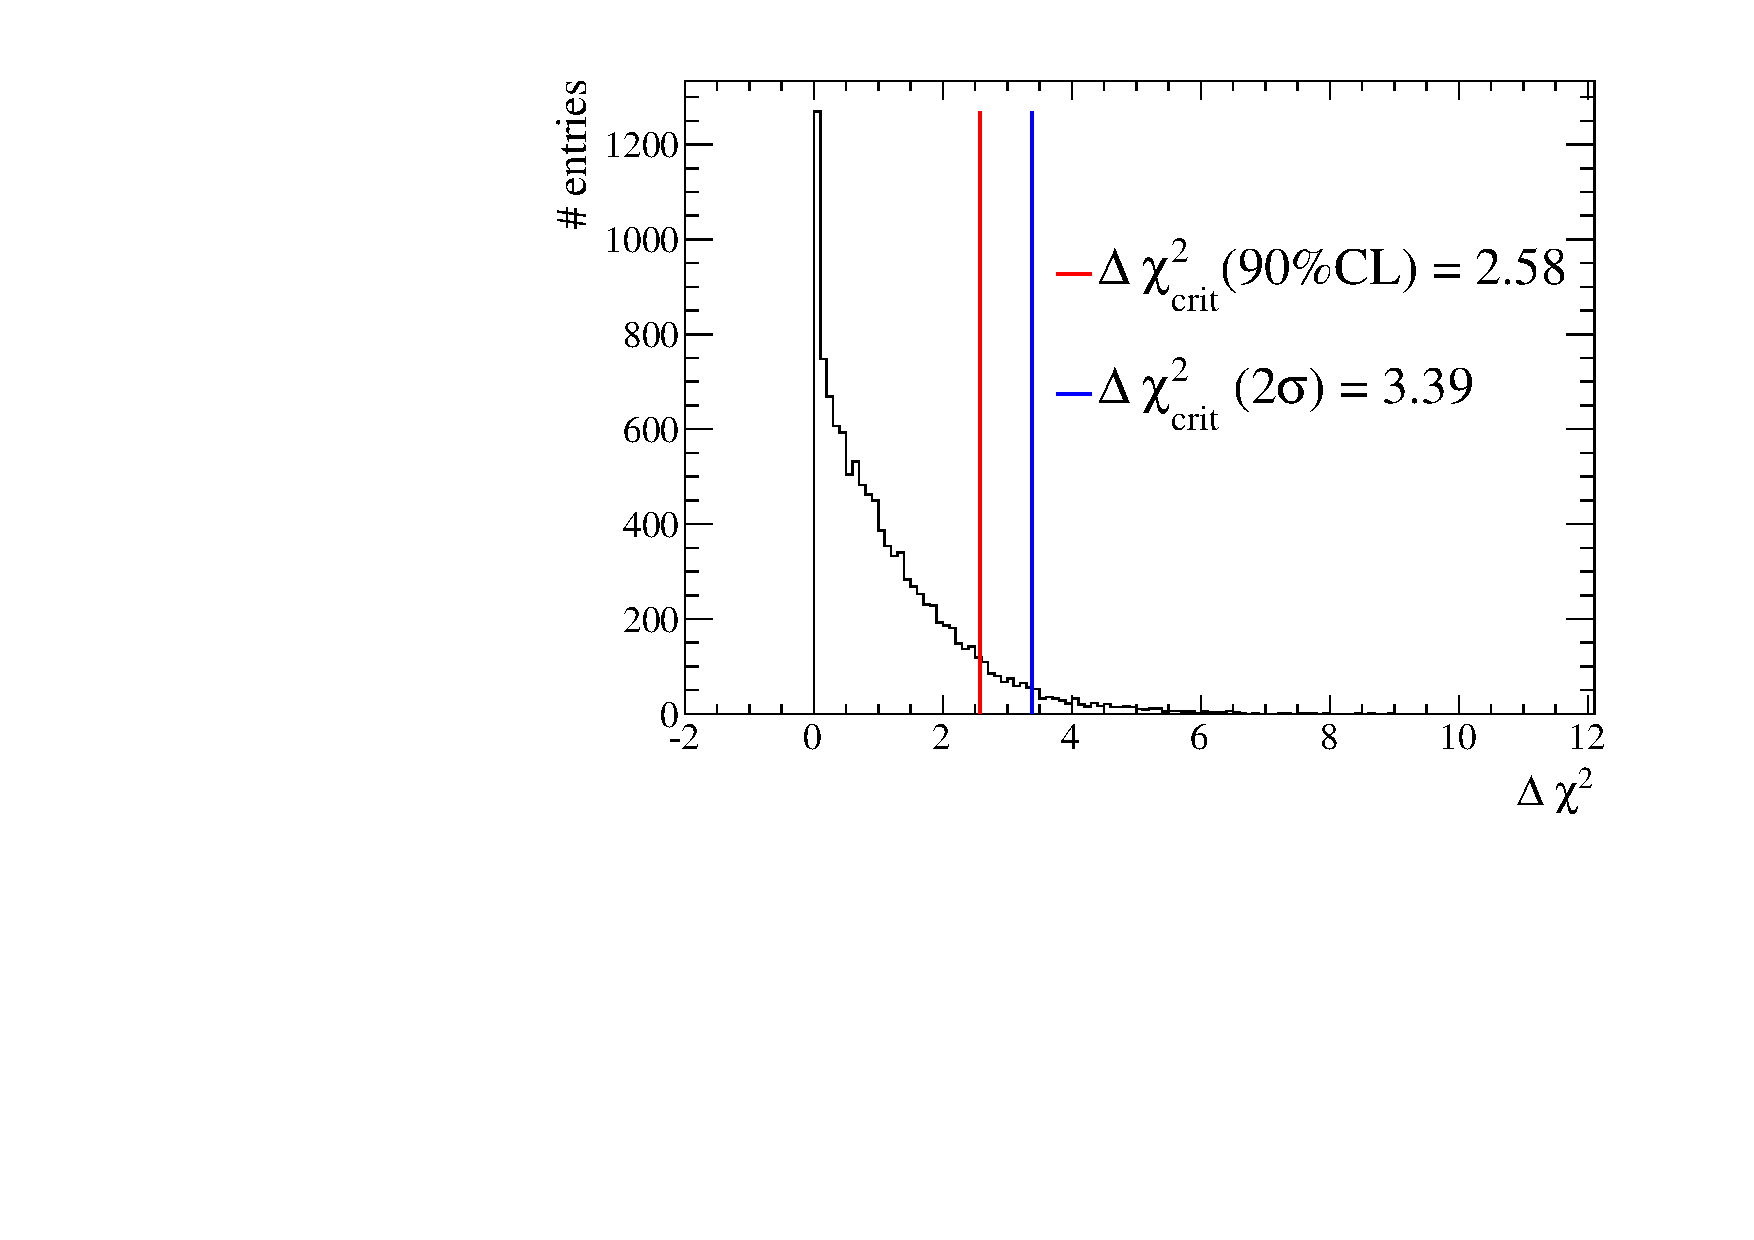
\includegraphics[width=0.9\textwidth]{./joint_plots/coverage_fc/coverage_run17c/Run17_deltachisq_glob_deltacp_0_normal.pdf}
\caption{$\Delta \chi^2$ distribution.
$\delta_{CP}^{true} = 0$.}
\end{subfigure}
\begin{subfigure}[b]{0.49\textwidth}
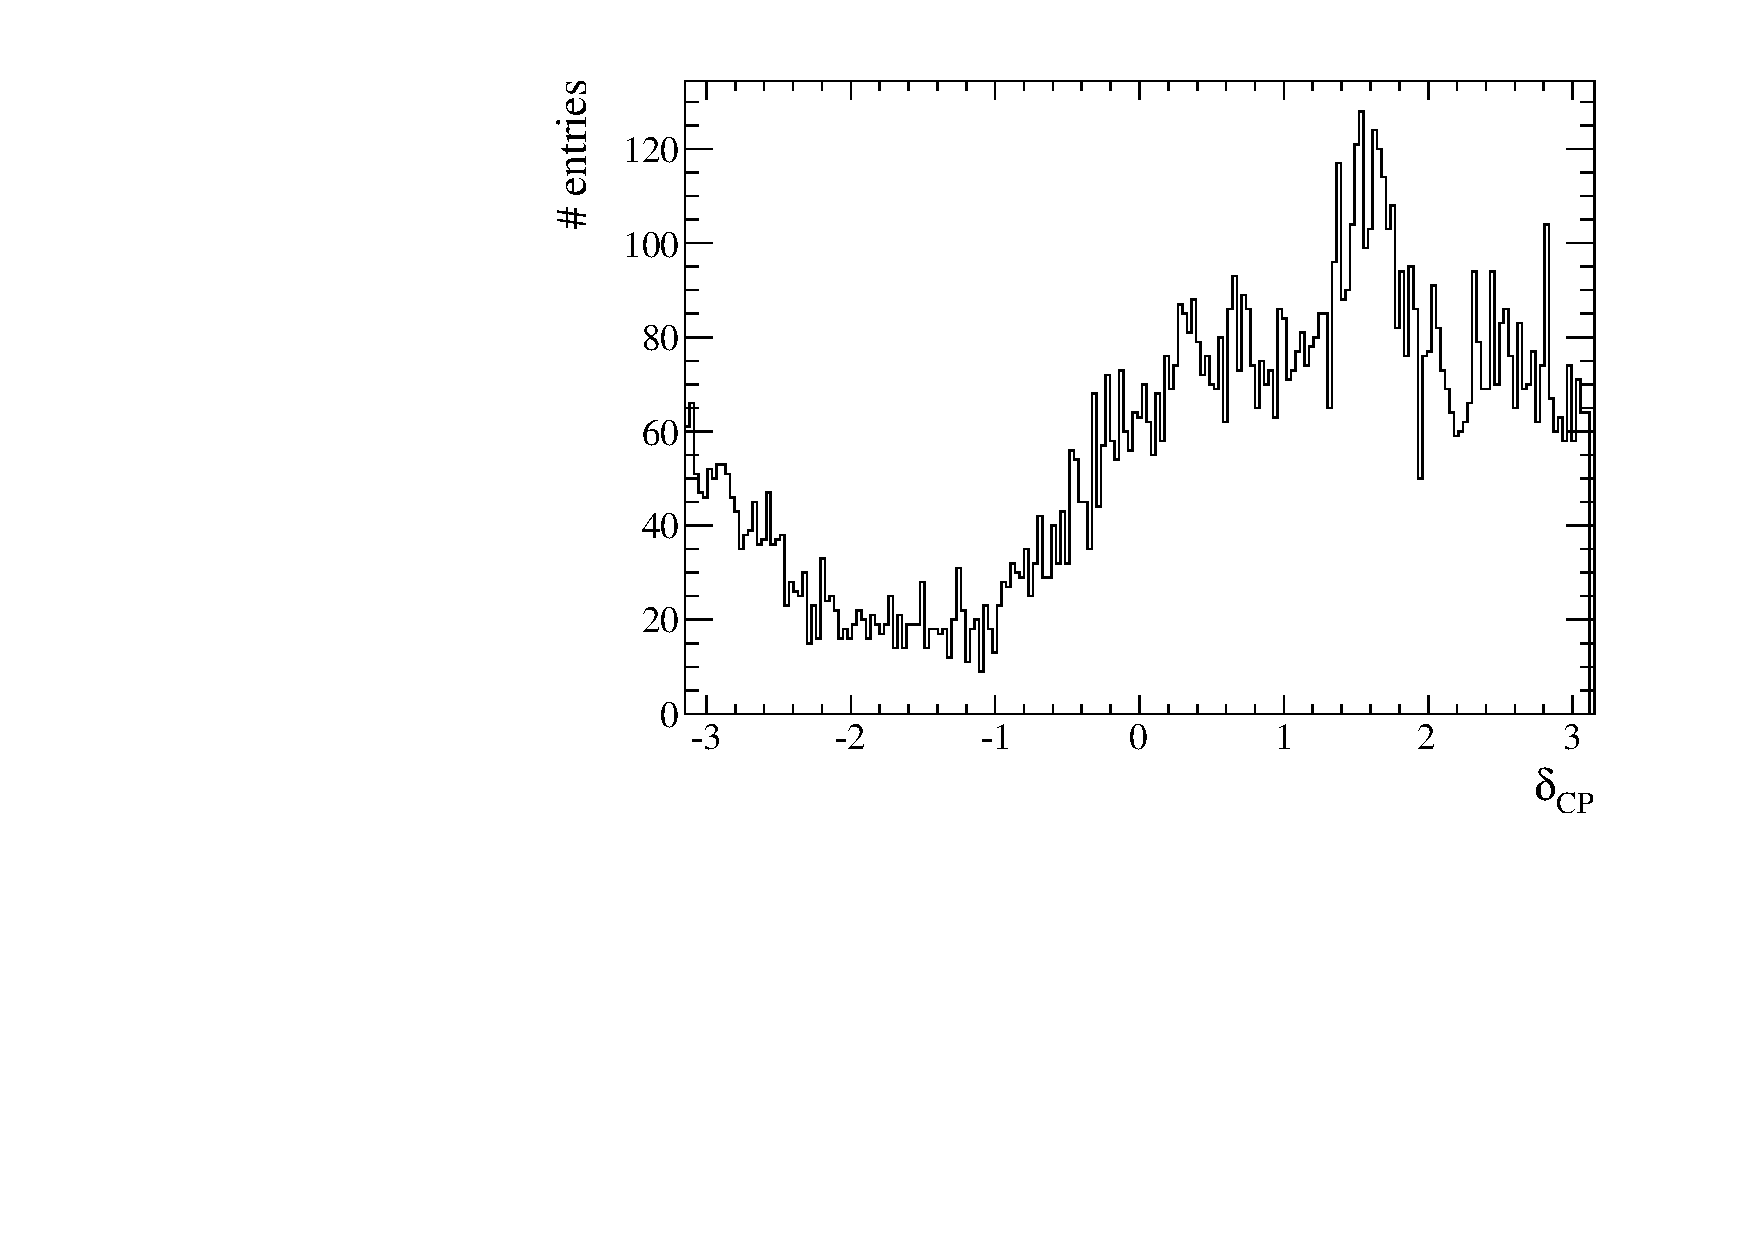
\includegraphics[width=0.9\textwidth]{./joint_plots/coverage_fc/coverage_run17c/Run17_cbestfit_deltacp_p1p571_normal.pdf}
\caption{Best-fit distribution of $\delta_{CP}$. $\delta_{CP}^{true} = +\pi/2$.}
\end{subfigure}
\begin{subfigure}[b]{0.49\textwidth}
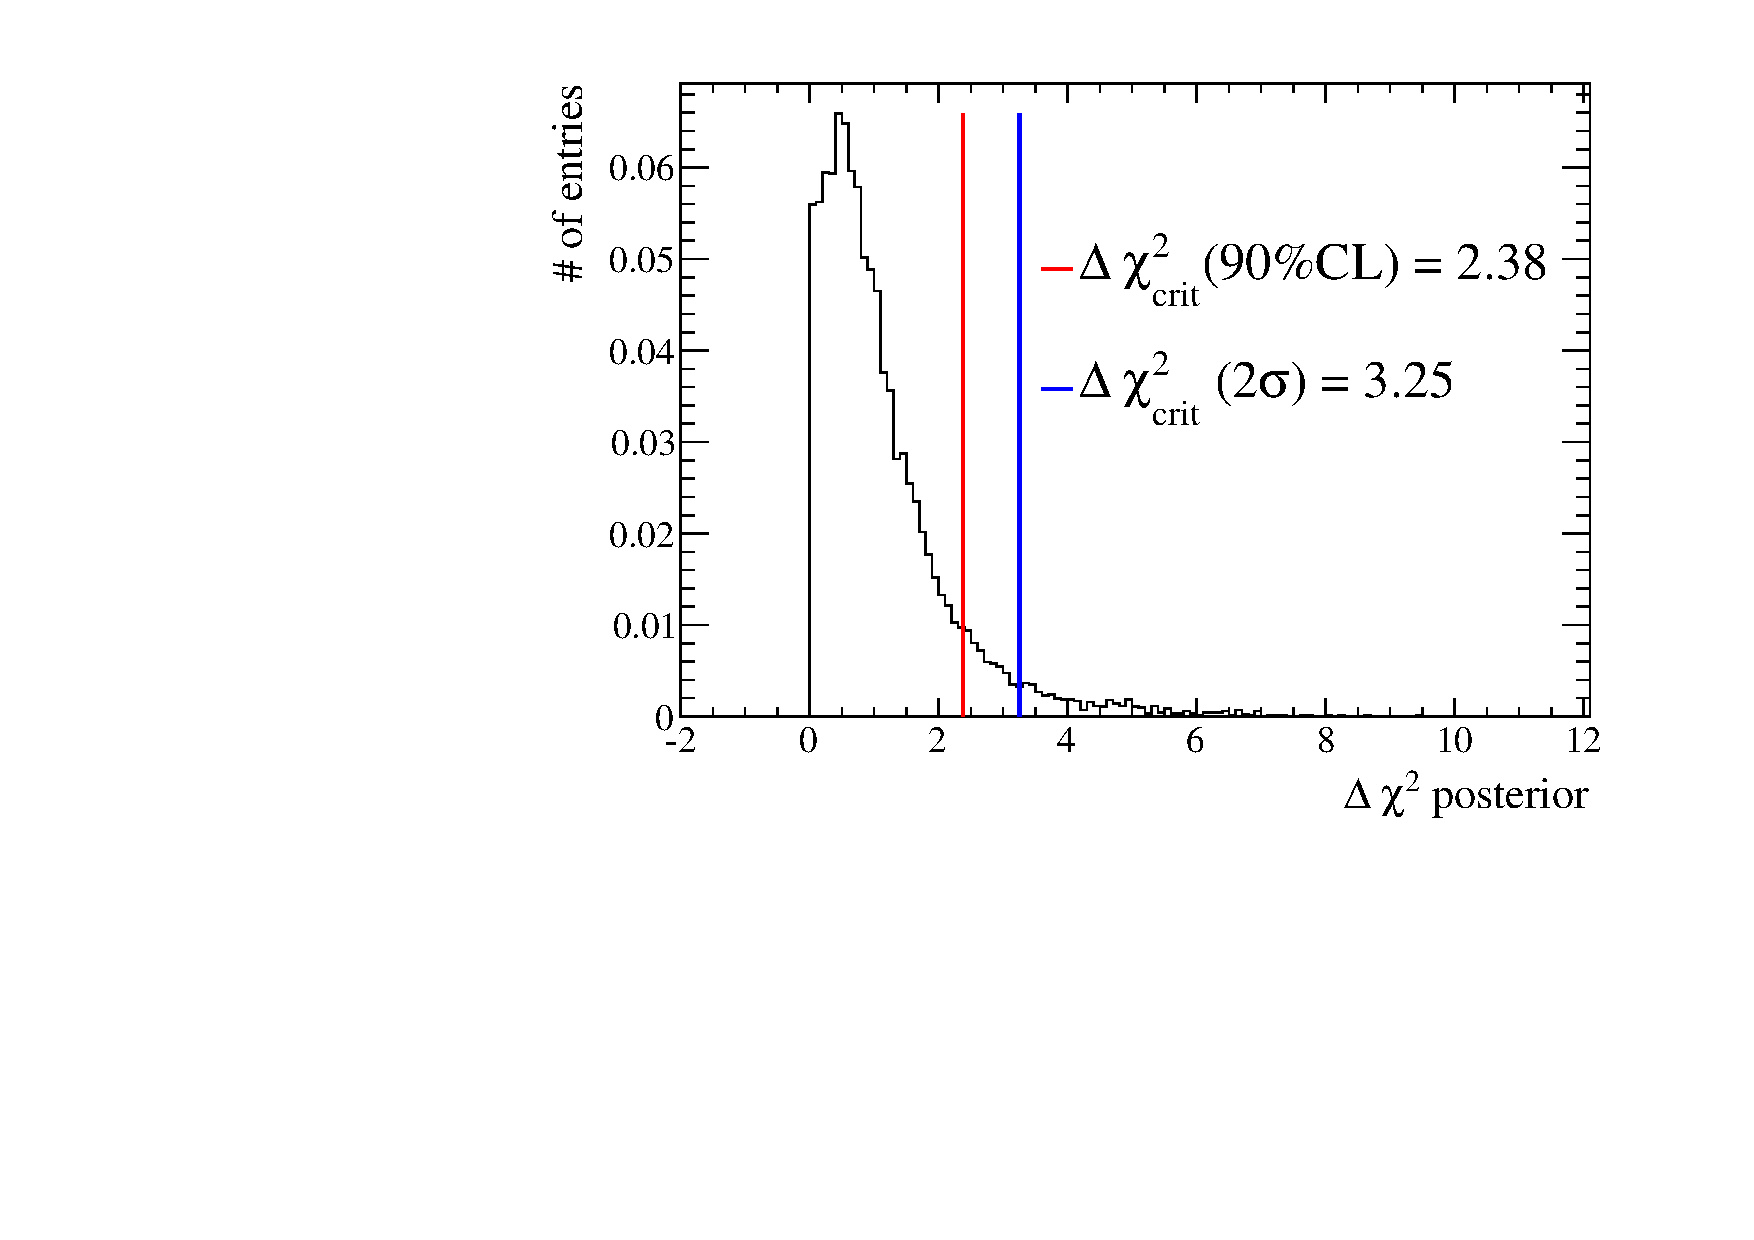
\includegraphics[width=0.9\textwidth]{./joint_plots/coverage_fc/coverage_run17c/Run17_deltachisq_glob_deltacp_p1p571_normal.pdf}
\caption{$\Delta \chi^2$ distribution.
$\delta_{CP}^{true} = +\pi/2$.}
\end{subfigure}
\caption {
Distributions of best-fit $\delta_{CP}$ (left) and $\Delta \chi^2$ (right).  
$10k$ toy experiments are performed
with true values of $\delta_{CP} = -\pi/2, 0, +\pi/2$, 
assuming normal hierarchy and applying the reactor constraint.
Both the mass hierarchy and $\delta_{CP}$ are profiled in the fit.
All the other oscillation parameters are marginalised.
The statistics corresponds to the Run 1-7c data set.
}
\label{fig:dchisq_bestfit_dcp_run17c}
\end{figure*}



\clearpage



%In \cref{fig:critval_comparision_run17b_run17c} the critical values obtained with the Feldman-Cousins method
%for both Run 1-6 and Run  1-7c statistic are shown.
%The critical values at both 90\% and $2\sigma$ CL are computed
%for both the mass hierarchies and the following true values of $\delta_{CP}$: 
%$-\pi$, -2.356, $-\pi/2$, -0.785, 0, +0.785, $+\pi/2$, -2.356, $+\pi$. 
%As already shown in \cref{tab:critval_0_pmhalfpi_run17c} and \cref{fig:dchisq_bestfit_dcp_run17c},
%the behavior of the critical values for Run 1-6 and Run 1-7c are quite similar, 
%given the fact that with Run 7c the additional amount of events is negligible in the neutrino mode $e$-like sample 
%(fewer than 0.5 event)
%and small in the antineutrino mode $e$-like sample (fewer than 3 events).



%\begin{figure*}[htb]
%\center
%\begin{subfigure}[b]{0.49\textwidth}
%%
\includegraphics[width=0.9\textwidth]{./images/missing_plot-eps-converted-to.pdf}
%%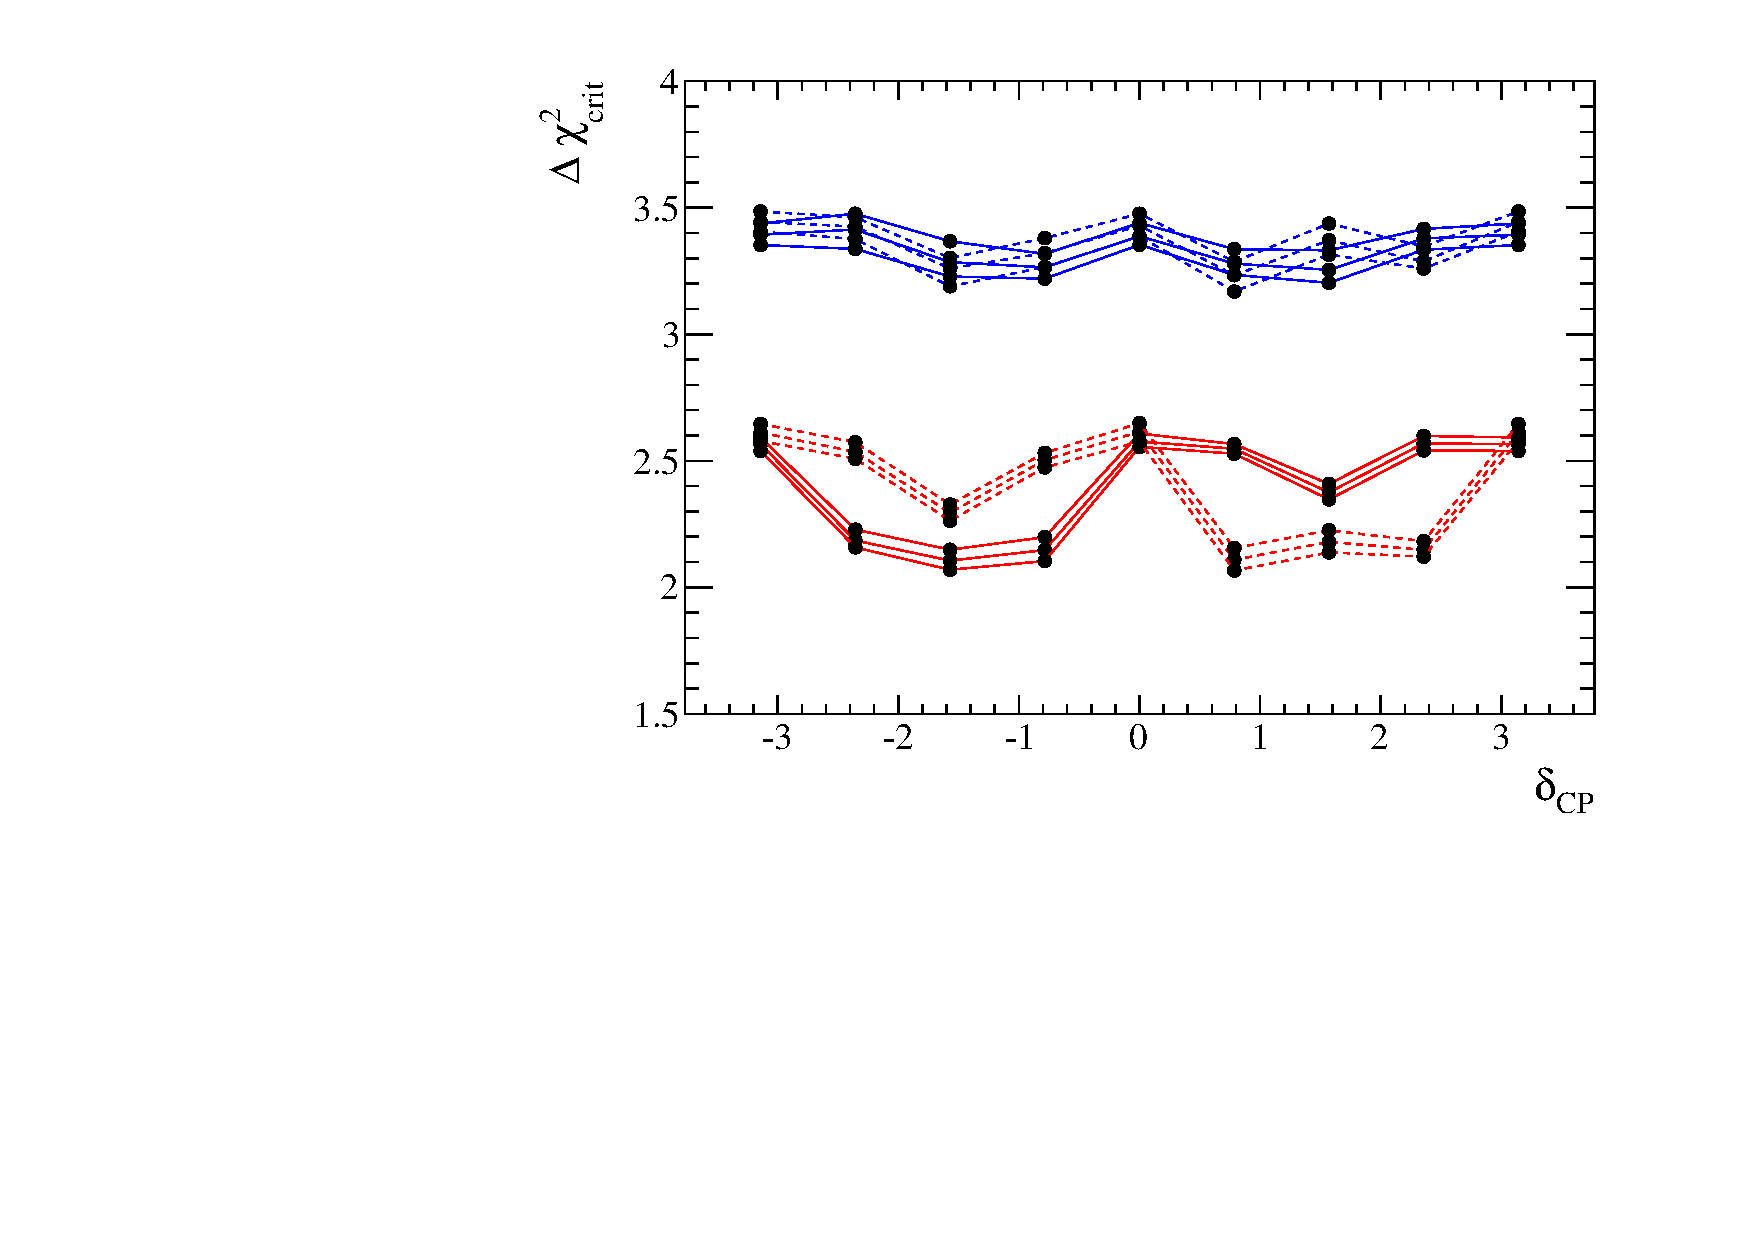
\includegraphics[width=0.9\textwidth]{./joint_plots/coverage_fc/fc_run17c/critical_values_run17c_fluxtun_run17b.pdf}
%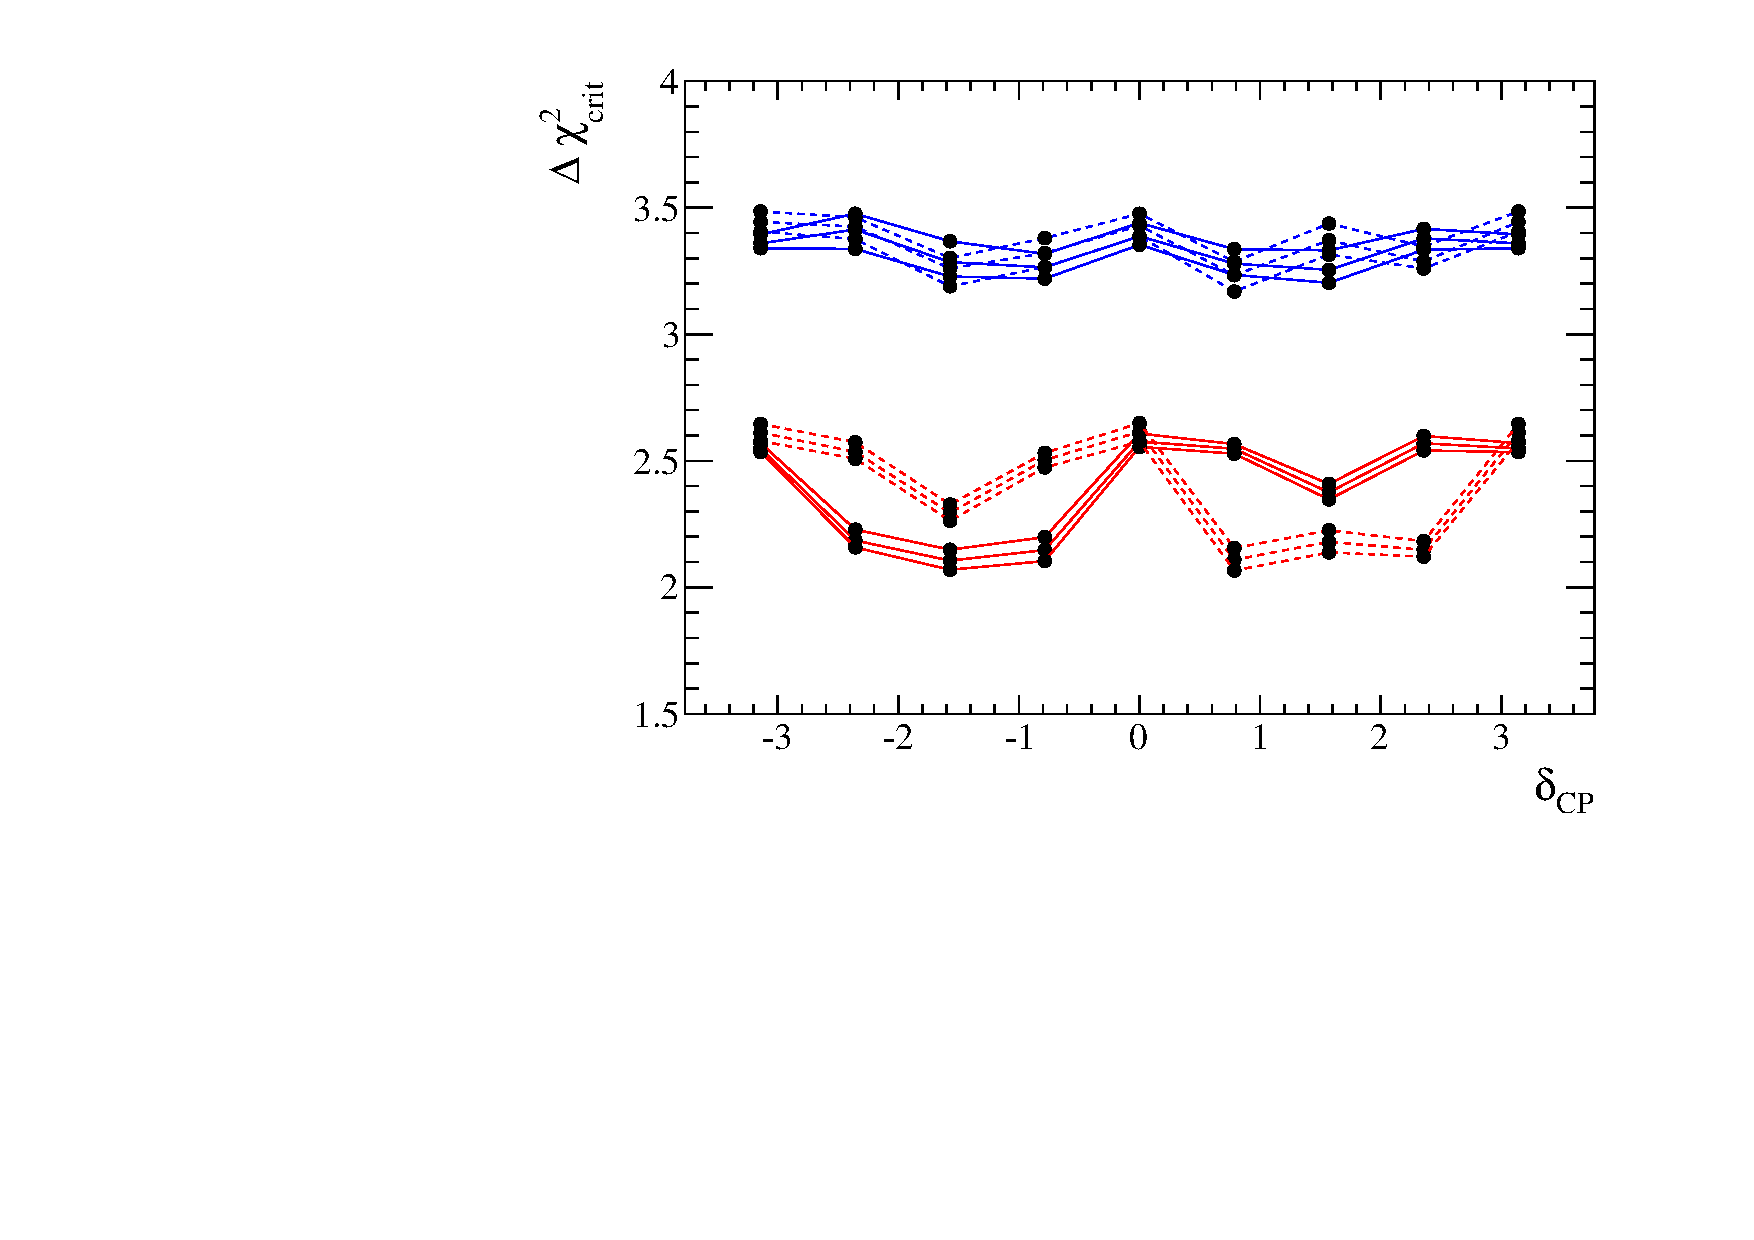
\includegraphics[width=0.9\textwidth]{./joint_plots/coverage_fc/fc_run17c/critical_values_run17c_fluxtun_merge_dcp_3p142.pdf}
%\caption{Critical values obtained with the Feldman-Cousins method for Run 1-7c statistic}
%\end{subfigure}
%\begin{subfigure}[b]{0.49\textwidth}
%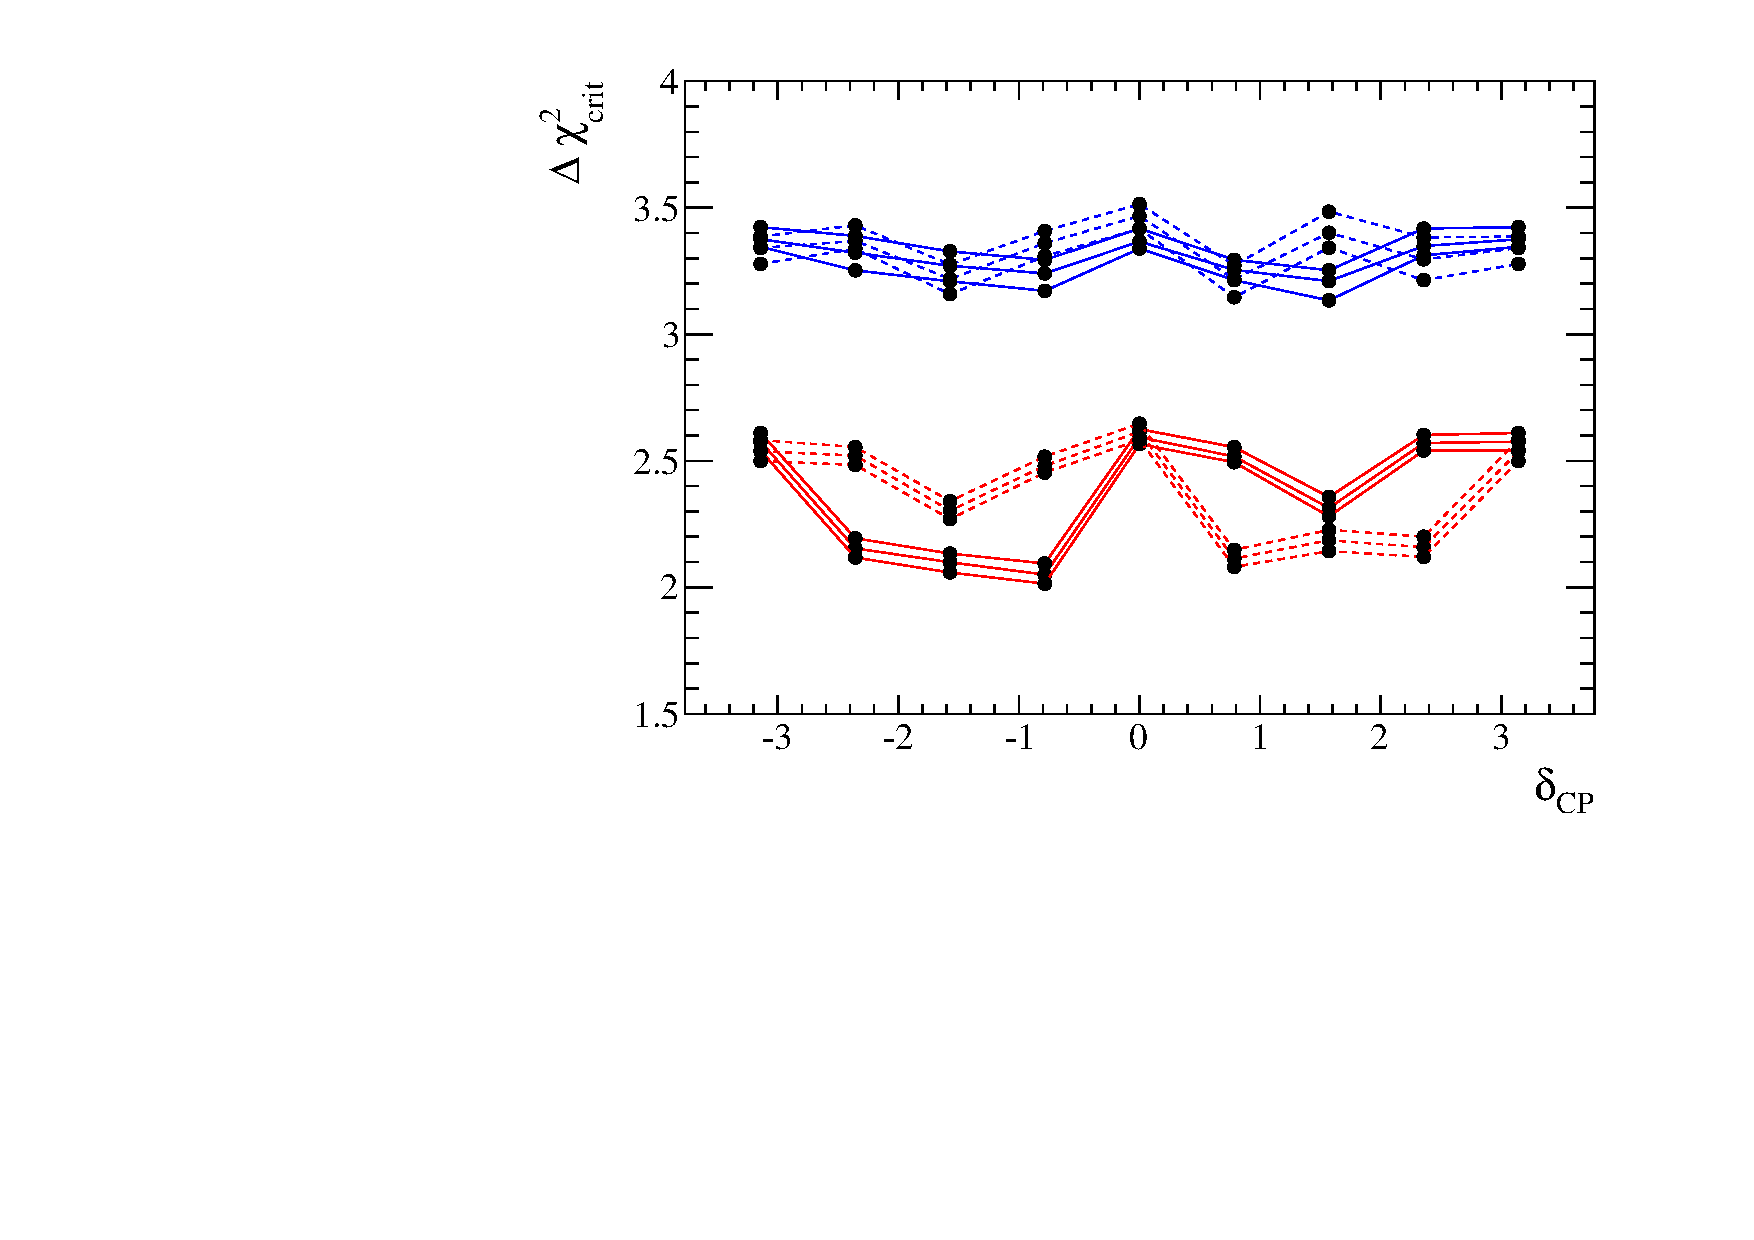
\includegraphics[width=0.9\textwidth]{./joint_plots/coverage_fc/fc_run17b/critical_values_fluxrun16.pdf}
%\caption{Critical values obtained with the Feldman-Cousins method for Run 1-7b statistic}
%\end{subfigure}
%\caption {
%Critical values obtained with the Feldman-Cousins method for Run 1-7c and Run 1-7b statistic
%for several true values of $\delta_{CP}$ and both normal (solid line) and inverted (dashed line) hierarchy.
%Both 90\% (red) and $2\sigma$ (blue) CL critical values are shown.
%About $10k$ toy experiments are performed for each point except $\delta_{CP} = \pi$ - normal hierarchy,
%for which $28k$ toy experiments are performed.
%All the other oscillation parameters are marginalised.
%The $\pm1 \sigma$ error on the critical values is shown as well
%and is represented by the lowest and highest set of critical values, with the same color of the central ones.
%}
%\label{fig:critval_comparision_run17b_run17c}
%\end{figure*}


\clearpage

\subsection{Validation of the minimisation algorithm}
\label{sec:minim_algorithm_run17c}

For each true value of $\delta_{CP}$, where the critical value is performed using the Feldman-Cousins method,
and normal hierarchy, 5000 fits were performed on fake data sets of the same type as used for Feldman-Cousins.
About all the fits except X found the global minimum.



\clearpage
